% ---------------------------------------------------------------------------
% R270 relocation target.  Every paragraph, table and footnote below was moved
% here VERBATIM (modulo cross-reference wording) from the main text so that the
% main text fits the ICLR 9-page limit.  Nothing was deleted: no ablation, seed,
% error bar, statistic or disclosure was dropped, and no number was changed.
% Provenance of each block is recorded in the comment above it.
% ---------------------------------------------------------------------------

\section{Extended Related Work and Contribution Boundary}
\label{app:related}
% Relocated from main-text Section 2 (02_related.tex, frozen face eada3e87).

\paragraph{Token-axis KV reduction.}
StreamingLLM keeps recent tokens and attention sinks~\citep{streamingllm}; H2O
keeps heavy hitters~\citep{h2o}; SnapKV predicts important positions from an
observation window~\citep{snapkv}; and PyramidKV varies the token budget across
layers~\citep{pyramidkv}.  These methods choose which token states to retain.
CoMem instead retains every token of a selected chunk at only one depth, so its
storage reduction is on the layer axis and does not imply that the external
store is fixed-size.  Layer-Condensed KV compresses the cache on the same layer
axis, sharing one condensed KV computed at a shallow depth across the upper
layers~\citep{lckv}, but it keeps a state for every token and performs no
top-$k$ retrieval, so its read still grows with retained tokens.  CoMem likewise
stores at a single depth but only for selected chunks and recomputes the upper
band with full cross-pack attention, bounding the read at fixed $k,c$.
YOCO shares one global cache across a decoder--decoder architecture rather than
storing retrieved per-chunk residual tensors~\citep{yoco}.  These layer-axis
designs motivate the comparison but are not implemented in our harness; the
paper's empirical claims are therefore internal matched controls, not a
performance ranking over prior systems.

\paragraph{Retrieval and cached blocks.}
Landmark Attention and Focused Transformer learn mechanisms for selecting
distant content~\citep{landmark,longllama}.  Serving systems such as CacheBlend
and RAGCache reuse KV for retrieved chunks and selectively repair cross-chunk
interactions~\citep{cacheblend,ragcache}.  CoMem shares their retrieval-first
view but stores a layer-$j$ activation rather than full-layer KV, then
recomputes the complete upper band with full cross-pack attention.  BM25 is an
external, non-differentiable selector rather than a learned contribution.
InfLLM keeps distant content in memory blocks that use unit/separate positions
and anchors the relevant blocks into the current segment, selecting blocks by
attention~\citep{infllm}.  CoMem shares the position-remap idea (fresh
contiguous positions for retrieved layer-$j$ activations) but selects chunks by
external BM25 rather than attention, stores a single-layer activation instead of
a unit-positioned block summary, and recomputes the complete upper band with
full cross-pack attention rather than attending to compressed anchors.
RETRO injects retrieved neighbors through deep cross-attention
\citep{retro}; Memorizing Transformers query an external $k$NN memory from a
single layer~\citep{memorizingtransformers}; Prompt Cache reuses modular prompt
segments through a position-remapping schema~\citep{promptcache}; and
Unlimiformer scales retrieval into encoder--decoder cross-attention
\citep{unlimiformer}.  These are closest on retrieval or reusable state, but
none couples a one-depth per-token store with fixed top-$k$ selection and full
upper-band recomputation.

\paragraph{Intermediate-state restoration.}
HCache restores evicted model state from intermediate activations, primarily as
a serving mechanism without document retrieval~\citep{hcache}.  KV-Direct shows
that a residual stream determines keys and values and can replace full-layer KV
when all retained tokens are reconstructed~\citep{kvdirect}.  CoMem combines
partial-depth recomputation with top-$k$ retrieval; unlike KV-Direct, it does
not retain all tokens in the active read, and unlike HCache it explicitly
selects chunks.  This combination is the contribution boundary.  We do not
claim the individual ingredients, numerical exactness for relocated $j>0$
states, or a system-level constant-memory store.  Training representations for
KV compressibility~\citep{kvcat} and CompressKV's semantic-retrieval-head-guided
token eviction~\citep{compresskv} are complementary token/representation-axis
approaches.  We treat Qasim et al.'s KV-Direct, Gelberg et al.'s
representation-training study, and Lin et al.'s CompressKV as 2026 arXiv
preprints~\citep{kvdirect,kvcat,compresskv}; CoMem was developed independently,
and its contribution boundary does not rely on any one of them.

\paragraph{Direct answers to the nearest-neighbor questions.}
\textbf{Which proposal is nearest?} Layer-Condensed KV~\citep{lckv} shares the
core idea of caching at a single shallow depth; HCache~\citep{hcache} and
KV-Direct~\citep{kvdirect} share the restoration-by-intermediate-state idea.
\textbf{What does it lack?} All three either let the read grow with retained
tokens (Layer-Condensed KV, and reconstruction-based KV-Direct when all tokens
are retained) or omit top-$k$ selection (HCache), and none measures cache-depth
fidelity under a fixed retrieval.  \textbf{Which falsifiable gap do we fill?}
A matched, preregistered measurement that fixes retrieval and varies only
cached depth, exposing that the depth cache---not retrieval---carries the
read-out quality loss.  This is a measurement/negative-result contribution; we
do not claim to outperform these designs on absolute benchmark scores, and in
the body the author's full-depth re-forward control is labeled as such, not as
an implementation of any of them.

% Relocated from main-text Section 3 (tab:method-boundary, 04_methodology.tex).
\begin{table*}[t]
\centering
\small
\setlength{\tabcolsep}{3pt}
\begin{tabular}{@{}>{\raggedright\arraybackslash}p{0.17\textwidth}
>{\raggedright\arraybackslash}p{0.18\textwidth}
>{\raggedright\arraybackslash}p{0.14\textwidth}
>{\raggedright\arraybackslash}p{0.19\textwidth}
>{\raggedright\arraybackslash}p{0.16\textwidth}@{}}
\toprule
\textbf{Method} & \textbf{Persistent object} & \textbf{Selection} &
\textbf{Model read as context grows} & \textbf{Recomputation} \\
\midrule
KV-Direct\newline\citep{kvdirect} & residual per retained token & none & grows with retained tokens &
full-depth reconstruction \\
HCache\newline\citep{hcache} & intermediate activation & none & grows with restored chunks &
upper-state restoration \\
YOCO\newline\citep{yoco} & one global decoder cache & none & grows with retained tokens &
shared cross-decoder cache \\
CacheBlend\newline\citep{cacheblend} & full KV for retrieved chunks & retrieval & fixed at fixed retrieval
budget & selective repair \\
Layer-Condensed KV\newline\citep{lckv} & single condensed KV at shallow depth & none &
grows with retained tokens & relax upper layers \\
InfLLM\newline\citep{infllm} & memory blocks (unit/separate positions) & attention & anchors
selected blocks & attend to compressed anchors \\
\textbf{CoMem} & one layer's $c\!\times\!d$ residual tensor per chunk plus text
index & BM25 top-$k$ & fixed at fixed $k,c$ & full upper band \\
\bottomrule
\end{tabular}
\caption{Mechanism boundary.  CoMem's distinctive combination is top-$k$
retrieval plus upper-band recomputation from a one-layer activation store; it
does not subsume the individual retrieval, residual-caching, or restoration
ideas.}
\label{tab:method-boundary}
\end{table*}

\FloatBarrier

\section{Method Details}
\label{app:method-details}
% Relocated from main-text Section 3 (04_methodology.tex): the generation
% boundary and selector paragraphs.

\paragraph{Autoregressive generation boundary.}
The recorded 0.68\,s quantity ends after read/prefill.  During generation the
current reference path rebuilds the upper-band pack at each decoded token; it
does not reuse an upper-layer KV cache across decode steps.  Generated tokens
are appended after the query at fresh contiguous positions and pass through
the same $F_{[j,L)}$ band.  We therefore do not convert the recorded prefill
endpoint into an end-to-end decode or throughput claim.

\paragraph{Sink and query construction in the read pack.}
In Eq.~(2) the sink is one BOS state computed independently through $F_{[0,j)}$
and reused within the read; its lower-layer context is only that BOS token.  The
query is separately computed through $F_{[0,j)}$ with query-local positions and
occupies the final fresh pack positions after the retrieved chunks.

\paragraph{Selectors and cross-chunk interaction.}
The primary selector is one-pass BM25 with $k_1=1.5$ and $b=0.75$.  An
exploratory \texttt{iter\_bm25} variant performs CPU-only chain following:
round one uses the query, and later rounds re-query with raw tokens from the
previous round's newly selected chunks.  It performs no model read between
hops.  Full cross-pack attention is part of the CoMem read; a block-diagonal
upper-band recompute is an ablation, not the default.

\paragraph{Storage accounting.}
The hidden store scales as $O(Mcd)$ and the text index as $O(|x|)$; both grow
with context.  Under Qwen3-8B's grouped-query attention, one per-token
activation stores one eighteenth of the elements of the full layer-wise
key--value cache.  This is a persistent-storage rate reduction, not a
constant-size memory.  Table~\ref{tab:factorized}'s GPU peaks compare fixed
read with full-context prefill, not depth alone; no end-to-end
persistent-storage baseline arm is run.

\FloatBarrier

\section{Full Experimental Protocol}
\label{app:protocol-full}
% Relocated from main-text Section 4 (03_motivation.tex): the RULER, LongEval,
% invariance, depth-sweep and terminology blocks, and the cross-trial pairing
% audit paragraph with its footnote.

\paragraph{RULER fixed-$k$ study.}
We evaluate the RULER \texttt{niah\_single} serving sweep~\citep{ruler} at 8k--128k with the
official \texttt{string\_match\_all} metric.  CoMem and the full-context
reference share the backbone and scorer; their read primitives differ.  We
report Wilson 95\% binomial intervals~\citep{wilson}; the sample count and seed
are in Table~\ref{tab:protocol-matrix}.  These cells quantify a complete short read versus a
full-context read, so they reflect the combined effect of retrieval and
working-set reduction, not the independent contribution of depth caching.
Figure~\ref{fig:system-tradeoff}'s 100\% statement is restricted to this
\texttt{niah\_single} fixed-read sweep; it is a different subtask and sample
set from Table~\ref{tab:ruler-percell}'s
\texttt{niah\_single\_3}, not a claim about every matched RULER cell.

\paragraph{Matched RULER study.}
The depth-only RULER audit holds an oracle/retrieval-fixed selector constant and
compares the same items under $j=0$ and $j=12$ across the registered
family--length cells.  Table~\ref{tab:protocol-matrix} records the shards,
pooled sample count, seed, and generation cap.  Per-item
\texttt{string\_match\_all} is fractional recall; strict correctness requires
all references.  Table~\ref{tab:ruler-percell} reports the cells, the
separately registered pooled full-match audit and its descriptive exact test,
and the serving-sweep exception, while Table~\ref{tab:factorized} carries only
the cell-level macro row.  Fractional cell
means are not used to reconstruct binary identities or the pooled tally.

\paragraph{Read-out invariance check.}
A separately preregistered higher-cap qa1 check tests read-out invariance.  The
legacy terminal-punctuation control is absorbing and therefore does \emph{not}
support a load-bearing truncation diagnosis.  The effective at-cap proxy cuts
the better arm more often, so truncation cannot explain the direction.
Table~\ref{tab:invariance-diagnostics} preserves the cap, sample,
reader, and discordant-cell details and labels the post-hoc diagnostics.

\paragraph{LongEval protocol.}
We use the released LongEval lines-retrieval benchmark~\citep{longeval} over the
registered context range.  BM25 selects top-$k$ raw-text chunks under the
per-task settings in Table~\ref{tab:protocol-matrix} ($k\in\{4,6\}$,
not the $k{=}12$ used at qa1/RULER); the metric is exact recovery of the
first valid line identifier in the full output.  Samples were generated
separately for the $j=0$ and $j=12$ arms and are not in one-to-one
correspondence, so the pooled LongEval column is \emph{not} a same-retrieval
depth isolation.  We therefore use an unpaired two-proportion test, not
McNemar; Table~\ref{tab:factorized} reports the pooled estimate and test and
is labeled accordingly.

\paragraph{Depth-partition sweep protocol.}
The preregistered depth sweep uses the same byte-pinned reader, oracle
selector, and $n{=}100$/bucket/arm as the decisive study
(Table~\ref{tab:depthcurve}, Figure~\ref{fig:depthcurve}).  At both tested
context lengths, accuracy shows an overall downward trend in cached depth and,
pointwise without multiplicity correction, every tested point from $j{=}2$
onward is a significant paired loss against $j{=}0$ on the same samples
(the observed curve is not strictly monotone---one $1$\,pp adjacent reversal at
$j{=}8\!\to\!10$ at 4k is within sampling noise at $n{=}100$; we run no ordered-trend
test).  The 16k \texttt{dense} (stock full-context, no CoMem) and
\texttt{full-depth re-forward (no retrieval)} baselines show no
significant difference from $j{=}0$ at $n{=}100$ ($p{=}0.43$/$0.50$); this does
not prove equivalence, but the observed $\le$6\,pp deficit is far below the
observed depth-associated $\ge$29\,pp effect.  The per-depth values and the
same-run wall-clock are merged into Table~\ref{tab:depthcurve}; per-depth sweep
memory peaks were not recorded (Appendix~\ref{app:depthcurve-cost}), and the
separate matched 128k memory check is reported in Table~\ref{tab:factorized}.
Optional LoRA and MoE diagnostics with incomplete configurations remain in
Appendix~\ref{app:secondary} and do not support the main claim.

\begin{figure}[htbp]
    \centering
    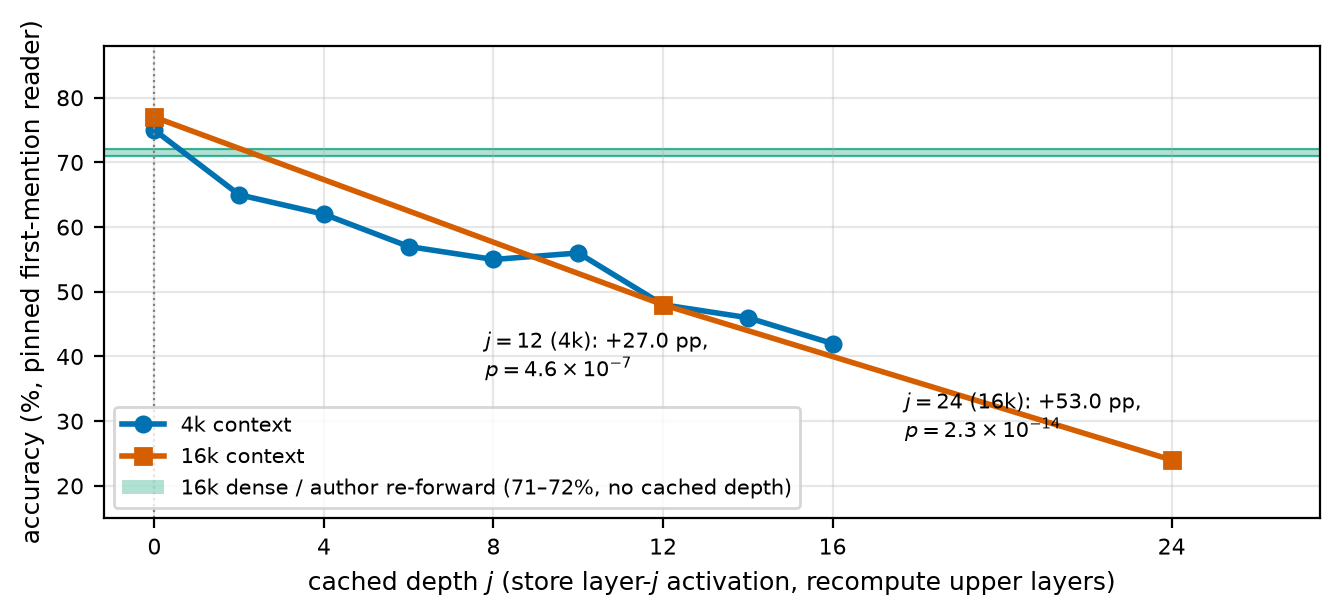
\includegraphics[width=0.86\columnwidth]{figures/depth_curve.png}
    \caption{\textbf{Complete depth-partition curve} (preregistered sweep;
    pinned reader, oracle selector, $n{=}100$/bucket/arm).  Accuracy trends
    downward with cached depth $j$ at both 4k (circles) and 16k (squares), and
    every tested point from $j{=}2$ onward is a significant paired loss against
    $j{=}0$; the trend is not asserted to be strictly monotone (the $1$\,pp
    reversal at $j{=}8\!\to\!10$ is within noise at $n{=}100$).  The shaded band
    is the 16k \texttt{dense} and \texttt{full-depth re-forward (no retrieval)}
    baselines, which have no cached depth and therefore no abscissa here; neither
    differs significantly from $j{=}0$ at $n{=}100$.  All tests are pointwise and
    uncorrected; the family-wise reading is in Table~\ref{tab:depthcurve}.}
    \label{fig:depthcurve}
\end{figure}

% Complete depth-partition curve from the frozen depth sweep
% (out/depth_sweep_full_v2_20260823_201948, prereg
% PREREG_DEPTH_SWEEP_FULL_ADDENDUM_V2_R158).  All acc values are n=100/bucket/arm
% under the byte-pinned robust_correct V2 reader (rev5, c5ba5674), independently
% reproduced by the external review from the raw CSVs.  Paired p is exact
% McNemar on discordant pairs vs the j=0 arm of the same context length.
% Operating points: 4k (j=0..16) and 16k (j=0/12/24 plus dense and re-forward
% baselines); 16k is the operating point, NOT 32k (no 32k claim).
%
% R270: merged with the former appendix wall-clock table (tab:depthcurve-cost)
% so that the eight duplicated arms appear once.  Every wall-clock second that
% table carried is preserved: the deeper-arm values are the new column and the
% two matched j=0 references (465.6 s at 4k, 528.5 s at 16k) are in the caption.

\begin{table}[t]
\centering
\small
\setlength{\tabcolsep}{4pt}
\begin{tabular}{@{}lccccc@{}}
\toprule
\textbf{ctx} & \textbf{$j{=}0$} & \textbf{deeper read} & $j{=}12$ & \textbf{$\Delta_{j0{-}j}$} & \textbf{exact $p$} \\
\midrule
% 4k axis: j0 vs each depth point
4k & 75.0 & $j{=}2$ & 65.0 & $+10.0$\,pp & $2.1\times10^{-2}$ \\
4k & 75.0 & $j{=}4$ & 62.0 & $+13.0$\,pp & $9.8\times10^{-4}$ \\
4k & 75.0 & $j{=}6$ & 57.0 & $+18.0$\,pp & $1.2\times10^{-4}$ \\
4k & 75.0 & $j{=}8$ & 55.0 & $+20.0$\,pp & $1.1\times10^{-5}$ \\
4k & 75.0 & $j{=}10$ & 56.0 & $+19.0$\,pp & $6.6\times10^{-5}$ \\
4k & 75.0 & $j{=}12$ & 48.0 & $+27.0$\,pp & $4.6\times10^{-7}$ \\
4k & 75.0 & $j{=}14$ & 46.0 & $+29.0$\,pp & $1.1\times10^{-6}$ \\
4k & 75.0 & $j{=}16$ & 42.0 & $+33.0$\,pp & $1.0\times10^{-7}$ \\
\midrule
16k & 77.0 & $j{=}12$ & 48.0 & $+29.0$\,pp & $1.3\times10^{-7}$ \\
16k & 77.0 & $j{=}24$ & 24.0 & $+53.0$\,pp & $2.3\times10^{-14}$ \\
\midrule
16k dense \textsuperscript{$\dagger$} & -- & -- & 71.0 & -- & $0.43$ \\
16k \mbox{re-forward} \textsuperscript{$\dagger$} & -- & -- & 72.0 & -- & $0.50$ \\
\bottomrule
\end{tabular}

\vspace{0.35em}
\begin{tabular}{@{}lcccccc@{}}
\multicolumn{7}{@{}l}{\emph{Same-run wall clock (s, $n{=}100$), recorded arms only}} \\
\toprule
\textbf{arm} & 4k $j{=}12$ & 4k $j{=}16$ & 16k $j{=}12$ & 16k $j{=}24$ &
16k \texttt{dense} & 16k re-forward \\
\midrule
seconds & 504.3 & 501.7 & 511.6 & 606.1 & 734.3 & 750.6 \\
\bottomrule
\end{tabular}
\caption{\textbf{Complete depth-partition curve (9+3 points, preregistered
sweep) with the same-run wall clock.}
Accuracy (\%) under the pinned first-mention reader ($n{=}100$/bucket/arm, oracle
selector); paired exact McNemar against the $j{=}0$ arm of the same length, which
shares the selected raw chunks (retrieval fixed) and the content-hash-verified
paired subset (Appendix~\ref{app:pairing-provenance}).  Every tested point from
$j{=}2$ onward is a significant paired loss against $j{=}0$ on the same samples;
the trend in $j$ is downward overall but we claim no strict monotonicity (the
single $1$\,pp reversal at $j{=}8\!\to\!10$ at 4k is within noise at $n{=}100$,
and each $p$ compares a depth to $j{=}0$, not to its predecessor).  The $p$
values are pointwise: under Bonferroni over the eight 4k comparisons the
shallowest $j{=}2$ cell ($p{=}2.1\times10^{-2}$) does not survive
$0.05/8{=}6.25\times10^{-3}$, so ``every point from $j{=}2$'' is pointwise, not
family-wise.  The load-bearing $j{=}12$ point is $+27.0$\,pp at 4k; at 16k the
$j{=}12$/$j{=}24$ losses are $+29.0$/$+53.0$\,pp.
\textsuperscript{$\dagger$}\texttt{dense} is stock full-context generation (no
CoMem) and \texttt{re-forward} the authors' full-depth re-forward without
retrieval (not an implementation of the published KV-Direct method): at 16k
neither differs significantly from $j{=}0$ at $n{=}100$ ($p{=}0.43$/$0.50$) --- a
non-rejection, not equivalence --- and their $\le6$\,pp deficit is the registered
bound on retrieval-side differences.  The lower block is the wall clock of the
same runs, so quality and cost are matched operation points: the matched $j{=}0$
references are $465.6$\,s at 4k and $528.5$\,s at 16k, and seconds were not
retained for the intermediate 4k depths $j{=}2$--$10$.  Per-depth peak memory was
not recorded (Appendix~\ref{app:depthcurve-cost}); data roots are in the protocol
matrix (Appendix Table~\ref{tab:protocol-matrix}).}
\label{tab:depthcurve}
\end{table}


\paragraph{Terminology used in the protocol and result tables.}
The \emph{primary reader} extracts the first task label; the \emph{stripped}
sensitivity first removes a model-generated option list, and the
\emph{answer-anchored} sensitivity searches only after the last answer cue.
A \emph{byte-pinned reader} is the frozen reader implementation identified by
its file hash; \texttt{split\_choices\_echo} is its single forward scan that
removes only a leading model-generated option enumeration, with no fallback.
A \emph{cap} is the maximum generated-token budget.  All reported $p$-values
identify the reader they were computed under and are shown in mathematical
notation.  Appendix Table~\ref{tab:protocol-matrix} records each primary run's
data root, generation cap, reader, sample count, and seed, with the caps listed
as separate runs rather than merged into a decision cell.  The \emph{oracle
selector} holds retrieved evidence fixed across arms.  \emph{At-cap} is a truncation
proxy, while \emph{floor-gated} marks a cell too weak to support the registered
claim.  The \emph{conditional convention range} is the min--max over the six
displayed reader/cap cells; the \emph{readout-identity envelope} instead assigns
unresolved answers adversarially.  Neither is an unconditional confidence
interval.

\paragraph{Five-arm cross-trial pairing audit.}
Pairing for the five-arm decomposition is by input content, not by row or
question string: \texttt{sample\_id = sha256(context+prompt+question)[:16]}.
This is the five-arm decomposition pairing (arms A/D/R/C/E), distinct from the
decisive single-supporting-fact three-arm pairing reported under
Appendix~\ref{app:pairing-provenance} (which cross-checks the pinned
$j{=}0$/$j{=}12$/re-forward qa1 cells).  At each
length, A/D/R/C (Trial 1895844) and the E-only repair (Trial 1896955) emit the
same ordered sequence of 100 unique IDs; qa1 has only four question strings
and six targets, so those strings are not pairing keys.  The failed first E
attempt stopped in argument parsing before creating an E directory or any
scorable output, so the repair run was not selected after seeing an E result.
An independent cross-trial audit of same-arm, same-code executions finds only
3 endpoint flips in 500 pairs (0.6\%; one-sided 95\% Clopper--Pearson upper
bound 1.54\%~\citep{clopper1934}, with $|\Delta\mathrm{acc}|\leq0.01$ per
unit).  By contrast, overturning the E--A exact test requires 8 directed flips
at 4k and 11 at 16k, 5--7$\times$ that worst-case noise bound.  Raw strings
change on 51--69\% of cross-trial rows and therefore have no discriminating
power; inference uses only the official-ruler endpoint and its paired $b/c$
counts.\footnote{The pairing, endpoint-noise, and tipping-point figures were
independently recomputed from the frozen trial trees in the third-party audit
records \texttt{r82\_pairing\_and\_crosstrial.txt},
\texttt{r82\_ENDPOINT\_CROSSTRIAL\_NOISE.txt}, and
\texttt{r82\_noise\_vs\_margin\_tipping.txt}.}

\paragraph{Reproducibility statement.}
Appendix~\ref{app:repro} records the frozen Qwen3-8B/bfloat16 software stack,
checkpoint and tokenizer hash prefixes, readers, selectors, seeds, generation
caps, hardware identities, and the limits of pairing verification.  The ethics
and generative-figure disclosure follows the reproducibility record.

\FloatBarrier

\section{Pairing Provenance on the Content-Hash-Verified Subset}
\label{app:pairing-provenance}
% New in this pass: R270 item (2) recompute.  No published value changes; the
% provenance status of the decisive cells does.

The preregistered sweep CSVs never emitted a separate \texttt{context\_sha256}
column (see the CSV column disclosure in Appendix~\ref{app:repro}).  They do
emit \texttt{sample\_id}, which the harness defines as the 16-hex prefix of
\texttt{sha256} over the full formatted model input, i.e.\ over the
concatenation of context, prompt, and question
(\texttt{eval/babilong.py} line 242).  That column is therefore itself a
content hash, and we re-ran the preregistered content-level join on it for
every decisive read-depth cell rather than leaving the field unverified.

Table~\ref{tab:pairing-join} reports the outcome.  In all 16 recomputed cells
each arm contributes 100 rows carrying 100 distinct content hashes, the two
arms share all 100 hashes (no arm-only and no duplicated hash), and the stored
question string agrees on every shared hash.  Recomputing each published cell
on that verified subset reproduces the printed accuracies, gaps, discordant
$b/c$ counts, and exact McNemar $p$ values \emph{exactly}: every comparison in
the recompute record is a match, so no number in this paper changes.  What
changes is the provenance status --- the decisive $j{=}0$ versus $j{=}12$ cells
are now certified to sit on a content-hash-verified paired subset rather than
on stored row order alone.  One limitation remains and is not repaired by this
recompute: the full 64-hex digest of the raw document text was never retained
as an independent artifact, so the join is over the formatted model input, not
over a separately stored document digest.

\begin{table}[htbp]
\centering
\footnotesize
\setlength{\tabcolsep}{4pt}
\begin{tabular}{@{}>{\raggedright\arraybackslash}p{0.30\textwidth}cccccc@{}}
\toprule
\textbf{cell group} & \textbf{cells} & \textbf{rows} &
\textbf{hashes} & \textbf{shared} & \textbf{arm-only} &
\textbf{q-mism.} \\
\midrule
mnt160 read-depth sweep (0k--8k)          & 5  & 100 & 100 & 100 & 0 & 0 \\
mnt512 decisive cell                      & 1  & 100 & 100 & 100 & 0 & 0 \\
depth sweep (4k $j{=}2$--$16$; 16k $j{=}12,24$) & 10 & 100 & 100 & 100 & 0 & 0 \\
\bottomrule
\end{tabular}
\caption{\textbf{Content-hash join for every decisive read-depth cell.}
The join key is the harness \texttt{sample\_id}, a 16-hex \texttt{sha256}
prefix over the full formatted model input.  \emph{rows} and \emph{hashes} are
per arm (rows contributed and distinct content hashes); \emph{arm-only} counts
hashes present in one arm and absent in the other; \emph{q-mism.}\ counts shared
hashes whose stored question string disagrees between arms.  No hash is
duplicated within an arm in any cell.  Every cell is a complete $100/100$
overlap, so all read-depth values in Tables~\ref{tab:depthcurve}
and~\ref{tab:readdepth-main} are computed on the verified paired subset, and the
recomputed values match the published ones cell by cell.}
\label{tab:pairing-join}
\end{table}

\FloatBarrier

\paragraph{Pairing-free floor for the load-bearing cell.}
Because a reviewer cannot audit the retired raw contexts directly, we also
report the estimate that survives with \emph{no} pairing assumption at all.
Treating the 4k pinned cell as two independent binomial arms
($75/100$ versus $48/100$) gives a $+27.0$\,pp difference with pooled
$z=3.924$ and two-sided $p=8.7\times10^{-5}$, and a Newcombe square-and-add
interval of $[+13.6,+39.1]$\,pp computed with the pairing correlation set to
zero.  That interval is deliberately wider than the paired constructions in
Table~\ref{tab:paired-cis}, which use the observed discordance: the paired test
is the efficient estimator, and the unpaired two-proportion result is the
assumption-free bound.  Both exclude zero, so the direction does not depend on
the pairing evidence.  The same construction applied to the mnt512 decisive
cell gives $[+10.7,+36.1]$\,pp (pinned) and $[+10.2,+34.8]$\,pp (stripped),
again wider than and consistent with the paired intervals.

\FloatBarrier

\section{Relocated Serving Record and Figures}
\label{app:figures}
% Relocated from the main text under the R270 page budget.  The table and both
% figures are unchanged: no row, datum or caption number was dropped, and the
% third serving panel of the old figure is now the recorded read/prefill rows of
% Table~\ref{tab:factorized}.

Table~\ref{tab:factorized} is the complete measured-quantity record for the
serving estimand, and Figures~\ref{fig:system-tradeoff} and~\ref{fig:readdepth}
are the serving overview and the read-depth length profile.  All three are
supporting views of Section~\ref{sec:serving} and Section~\ref{sec:readdepth};
the load-bearing read-depth estimates remain in Table~\ref{tab:readdepth-main}.

\begin{table}[htbp]
\centering
\footnotesize
\setlength{\tabcolsep}{3pt}
\begin{tabular}{@{}>{\raggedright\arraybackslash}p{0.14\textwidth}
>{\raggedright\arraybackslash}p{0.25\textwidth}
>{\raggedright\arraybackslash}p{0.24\textwidth}
>{\raggedright\arraybackslash}p{0.28\textwidth}@{}}
\toprule
\textbf{Block} & \textbf{Arm / estimand} & \textbf{Protocol} & \textbf{Recorded result} \\
\midrule
\textbf{128k serving} & Full context & all raw tokens; all layers & 72.7\,s read; 71.4\,GB \\
& Full context at 8k & shortest recorded full-context read & 1.28\,s read \\
& Matched $j=0$ timing & selected raw tokens; same $k$ & 0.94\,s read \\
& CoMem $j=12$ & selected $h_{12}$; same $k$ & 0.68\,s read; 18.29\,GB \\
& Balanced break-even & $W=6.65$\,s, $G=1$; decode excluded & $Q^{\star}=25.58$ reads/document ($\approx26$) \\
\midrule
\textbf{E1 matched memory} & $j=0$ & read length 6,657; median of 3 & 18.2\,GB \\
& $j=12$ & same read/hardware; median of 3 & 17.9\,GB \\
& Depth-attributed saving & $(12/36)B_{\mathrm{KV}}\,\textit{read\_len}$ & 0.3\,GB (0.2--0.4\,GB) \\
\midrule
\textbf{Separate quality} & RULER macro, \emph{estimand mixture} & unweighted mean over 15 cells: 3 fractional \texttt{string\_match\_all} recall, 12 strict-binary & 99.19 $\to$ 96.07; gap 3.12\,pp \\
& RULER strict-binary pooled drop & 1,500 item pairs, $(c-b)/n$ & $82/1500=5.47$\,pp \\
& RULER \texttt{niah\_single} fixed read & serving sweep, $n{=}50$/cell, 8k--128k & 100\% at every in-regime length \\
& LongEval & unpaired, $n=500$ per arm; $k\in\{4,6\}$ & 97.2 $\to$ 69.0; 28.2\,pp [23.9,32.5]; $z=11.9$ \\
\bottomrule
\end{tabular}
\caption{\textbf{Measured quantities split by operating point.}  The serving
block is a whole-system retrieval comparison of recorded read/prefill endpoints;
E1 is the matched memory-only depth isolation, scoped to
\textit{read\_len}=6,657, and establishes no end-to-end or general memory
benefit.  The RULER macro row is explicitly an \emph{estimand mixture}: an
unweighted mean over 15 (task,\,length) cells of which three report fractional
\texttt{string\_match\_all} recall and the rest strict-binary correctness, so it
is not a single-estimand accuracy.  The comparable strict-binary quantity is the
pooled $5.47$\,pp drop; the item-level pooled exact test over 1,500 clustered
pairs is descriptive only and appears with its per-cell breakdown in Appendix
Table~\ref{tab:ruler-percell}.  The 100\% row is the \texttt{niah\_single}
serving sweep, a different subtask and sample set from that appendix table.
LongEval is unpaired with a different selector budget, so it is not a
same-retrieval depth isolation and its 95\% Wald interval assumes independent
binomial arms.  Timing dispersion was not retained; serving timings are medians
of three.}
\label{tab:factorized}
\end{table}

\begin{figure}[htbp]
    \centering
    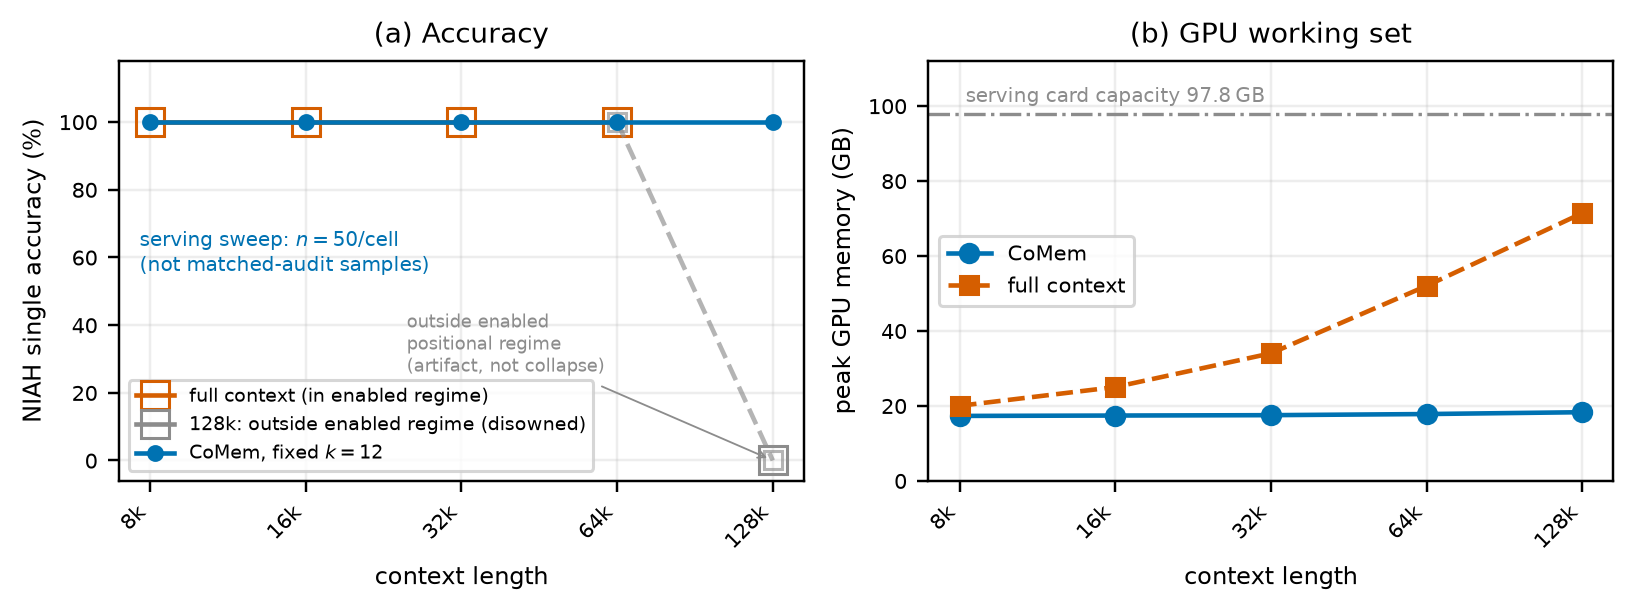
\includegraphics[width=\textwidth]{figures/system_tradeoff.png}
    \caption{\textbf{Fixed-$k$ preserves the short-read operating point while
    full-context cost grows.}  Panel (a) is the separate \texttt{niah\_single}
    serving sweep ($n{=}50$/cell), not Table~\ref{tab:ruler-percell}'s
    \texttt{niah\_single\_3}.  The 128k full-context point is greyed and
    annotated \emph{outside enabled positional regime}: it lies outside this
    checkpoint's enabled positional range and is disowned as a positional
    artifact, not a full-attention-collapse finding.  Panel (b) adds the
    97.8\,GB serving-card capacity line, below which full attention remains
    feasible at 128k (71.4\,GB).  The former read-time panel is now the recorded
    read/prefill rows of Table~\ref{tab:factorized}, because three endpoints are
    not a sweep.  The depth-axis quality cost is plotted in
    Figure~\ref{fig:depthcurve} and Table~\ref{tab:depthcurve} instead; these
    protocols are not one paired Pareto sweep.}
    \label{fig:system-tradeoff}
\end{figure}

\begin{figure}[htbp]
    \centering
    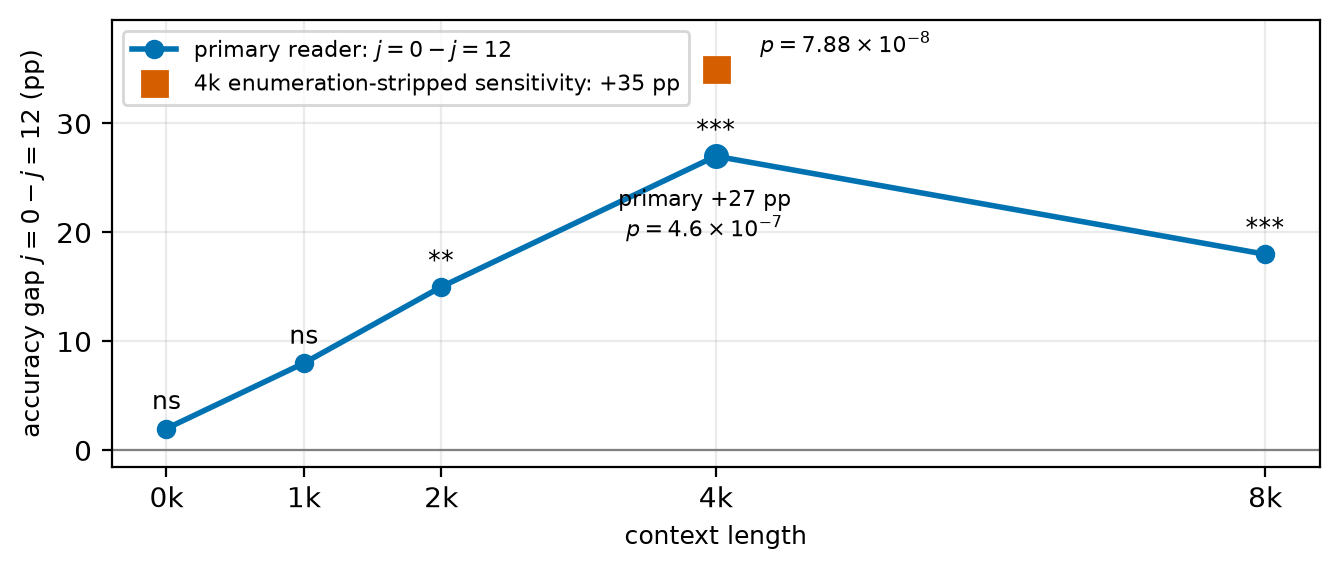
\includegraphics[width=\columnwidth]{figures/readdepth_qa1_gap.png}
    \caption{Primary-reader $j{=}0-j{=}12$ qa1 gaps over context length
    ($n{=}100$/bucket/arm, oracle selector).  The square is the
    enumeration-stripped sensitivity at the 4k decision cell.  The curve is
    not monotone; the load-bearing result is the pinned \emph{direction} and
    the $+27.0$/$+24.0$\,pp point pair on the same samples at the two caps.  The
    conditional convention range is in Table~\ref{tab:readdepth-decisive};
    neither is a claim of length-robust growth.  Symbols encode pointwise exact
    McNemar tests: ${*}\,p<0.05$, ${**}\,p<0.01$, ${***}\,p<0.001$, and
    ``ns'' $p\geq0.05$; no multiplicity correction is applied in this panel.}
    \label{fig:readdepth}
\end{figure}

\FloatBarrier

\section{Extended Limitations}
\label{app:extended-limitations}
% Relocated verbatim from the main-text Limitations section under the R270 page
% budget.  The main text keeps the load-bearing statements and points here; no
% caveat was removed.

\paragraph{Selection and uncertainty.}
The archived best-$k$ sweeps lack a validation/test separation, so we report
fixed $k=12$.  Primary RULER and qa1 cells have $n=50$ and $n=100$ under one
checkpoint and deterministic data seed.  The qa1 oracle selector isolates
depth but leaves its interaction with deployment BM25 unmeasured.  Overlapping
half-splits diagnose resampling stability, not independent replication; our
intervals do not cover checkpoint, model-family, or implementation variability.
No column literally named \texttt{context\_sha256} was emitted, so the
recomputed join uses the emitted \texttt{sample\_id} content hash and is
therefore over the formatted model input rather than over an independently
stored 64-hex document digest, which was never retained
(Appendix~\ref{app:pairing-provenance}); for the load-bearing cell we
additionally report the pairing-free two-proportion floor.

\paragraph{Scorer resolution of the five-arm deck.}
The official scorer collapses roughly six in ten raw-generation differences onto
a single label, so the $0/100$ endpoint agreement between arms (e.g.\ E and C) is
indistinguishability \emph{at label resolution}, not identity or inertness of a
deleted factor in the forward pass.  We therefore report the generation-layer
distinguishability counts alongside the endpoint discordance; the null is a
scorer-resolution statement only.

\paragraph{Composition boundary and the archived read adapter.}
The qa2 probe is not load-bearing: one cell is parser-invariant and non-floor;
the rest are negative-control, format-artifact, or floor-gated cells.  Appendix
Table~\ref{tab:composition-app} reports them, together with the registered
generation-cap sensitivity runs whose constant direction is consistent with the
gap not being created by generation budget alone; no length-robust claim
follows, and other format effects are not ruled out.  A self-distilled read
adapter appears in this workspace only as an archived configuration
(Appendix Table~\ref{tab:selfdistill-config}): it is not evaluated here and
carries no accuracy claim in this paper.
